%  \documentclass[DIV=12, a4]{scrartcl}
%\documentclass[12pt, a5]{scrartcl}
\documentclass[a4]{scrartcl}

\usepackage[
fancytheorems, 
noindent, 
%spacingfix, 
%noheader
]{adam}

% \usepackage{subfig}

% \setcounter{section}{-1}

\title{Groups}
% \subtitle{Adam Kelly}
\author{Adam Kelly, Lectured by Dr. A. Khukhro}
\date{Michaelmas 2020}

\begin{document}

\maketitle

\begin{abstract}
	This document is an account of the Cambridge Mathematical Tripos course `Groups', lectured by Dr. Ana Khukhro. in Michaelmas 2020.
	This is a work in progress, and is likely to to contain errors, which you may assume to be my own.
	% This document is a rather brief summary of the first three chapters of H. S. M. Coxeter and S. L. Greitzer's `Geometry Revisited'.
	% In no ways is this fleshed out, and in most cases just contains the important results and diagrams.
	% Specifically, it's purpose is to be somewhat of a reference which one can consult whilst attempting olympiad geometry problems.
\end{abstract}

\tableofcontents

\clearpage

\section{Groups}

\subsection{Definition}

In this section we will formally introduce the notion of a group, and we will consider some examples of groups along with their basic properties.

\begin{definition}
	A \vocab{group} is a set $G$ with a binary operation $*$ on $G$ such that:
	\begin{itemize}
		\item \emph{Identity}. $G$ has an \vocab{identity element} $e$ such that $e * g = g * e = g$ for all $g \in G$.
		\item \emph{Inverses}. Each element $g \in G$ has an \vocab{inverse}, that is, an element $g^{-1} \in G$ such that $g * g^{-1} = g^{-1} * g = e$.
		\item \emph{Associativity}. The operation $*$ is associative, that is $(g * h) * k = g * (h * k)$ for any $g, h, k \in G$. 
	\end{itemize}
\end{definition}

\begin{remark}[A pedantic point]
	In some cases, people will add an additional `closure' axiom, stating that if $g, h \in G$ then $g * h \in G$. However, this is redundant as it is implied by stating that $*$ is a binary operation on $G$. You must keep it in mind however when checking if something is a group.
\end{remark}
\begin{remark}[Bracketing]
	The `associativity' axiom means that we can write $g * h * k$ without specifying what order it should be done first.
\end{remark}

\begin{notation}
	It's proper to state that `$(G, *)$ is a group', but this is regularily abbreviated to saying `$G$ is a group', whenever the operation being used is clear.
\end{notation}

So that's what a group is, let's dive straight into some examples.

\begin{example}[Examples of Groups]
	The following are all examples of groups.
	\begin{enumerate}
		\item $G = \{e\}$, along with the binary operation $*$ satisfying $e * e = e$ (the `trivial group').
		\item $G$ being the set of symmetries of a shape, along with $g*h$ defined to be `performing $h$ followed by $g$' where $g, h \in G$ is a group.
		\item $(\mathbb{Z}, +)$, $(\mathbb{Q}, +)$ , $(\mathbb{R}, +)$  and $(\mathbb{C}, +)$ are all groups.
		\item The nonzero\footnote{You should consider why we need to exclude zero for $\mathbb{R}$ to be a group.} real numbers $\mathbb{R}\backslash \{0\}$ with multiplication is a group.
		\item $(\mathbb{R}, *)$ where $r * s = r + s + 5$ for any $r, s \in \mathbb{R}$ is a group.
		\item $\mathbb{Z}_n = \{0, 1, \dots, n - 1\}$ with addition modulo $n$ is a group.
		\item A vector space with vector addition is a group.
		\item The set of invertible $2 \times 2$ matrices with real coefficients, $GL_2(\mathbb{R})$ is a group with respect to matrix multiplication.
	\end{enumerate}
\end{example}
\begin{proof}[Proof Sketch]
	Check that each construction satisfies all of the axioms stated in the definition of a group.
\end{proof}

Let's also look at some structures that are \emph{not} groups.

\begin{example}[Non-Examples of Groups]
	The following are all \emph{not} groups.
	\begin{enumerate}
		\item $G = \{0, 1, 2, \dots, n - 1\}$ with addition.
		\item $(\mathbb{Z}, \times)$.
		\item $(\mathbb{R}, *)$ where $r * s = r^2 s$ for $r, s \in \mathbb{R}$.
		\item $G = \{0, 1, 2, \dots\}$ and the operation $*$ such that $m * n = |n - m|$ for $m, n \in G$.
	\end{enumerate}
\end{example}

\begin{notation}
	We often write $g \cdot h$ or $gh$ for $g * h$, where $*$ is the group's binary operation.
\end{notation}

\subsection{Direct Consequences of the Definition}

Let's look at some easy consequences of the group axioms.

\begin{proposition}
	Let $G$ be a group, and let $g$ be any element of $G$.
	\begin{enumerate}[label=(\roman*)]
		\item The identity element is unique.
		\item The inverse of $g$ is unique.
		\item If $g*h = g$, then $h * g = g$ and $h = e$.
		\item If $g * h = e$, then $h * g = e$ and $e = g^{-1}$.
		\item $(gh)^{-1} = h^{-1} g^{-1}$.
		\item $(g^{-1})^{-1} = g$.
	\end{enumerate}
\end{proposition}
\begin{proof}
	We will prove each in order.
	\begin{enumerate}[label=(\roman*)]
		\item Suppose that $e$ and $e'$ are both identity elements. Then
		$$
		e * e' = e \quad \text{and} \quad e * e' = e',
		$$
		hence $e = e * e' = e'$.
		\item Suppose that $g*h = e$ and $gk = e$. Then
		\begin{align*}
			g * h &= g * k \\
			\implies g^{-1} * g * h &= g^{-1} * g * k \\
			\implies h &= k.
		\end{align*}
		\item If $g * h = g$ then we have
		\begin{align*}
			g * h &= g \\
		\implies g^{-1} * g * h &= g^{-1} * g \\
		\implies h &= e.
		\end{align*}
		\item If $g * h = e$ then
		\begin{align*}
			g * h &= e \\
			\implies g^{-1} * g * h &= g^{-1} * e \\
			\implies h &= g^{-1}.
		\end{align*}
		\item We have
		$$
		(g*h) * (h^{-1} g^{-1}) = g * h * h^{-1} * g^{-1} = g * g^{-1} = e, 
		$$
		thus $(gh)^{-1} = h^{-1} g^{-1}$ by definition.
		\item Note that $g * g^{-1} = e$, so $g$ is the inverse of $g^{-1}$ which is unique by (ii), so $g = (g^{-1})^{-1}$.
	\end{enumerate}
\end{proof}

\begin{definition}
	A group $G$ is \vocab{abelian} (or commutative) if $\forall g, h \in G$, $g * h = h * g$.
\end{definition}

\begin{definition}
	A group $G$ is \vocab{finite} if it has a finite number of elements, and it is \vocab{infinite} otherwise. The number of elements of $G$ is the \vocab{order} of $G$, written $|G|$.
\end{definition}

\subsection{Subgroups}

Given any mathematical object, it's typically useful to know about its `subobjects'.

\begin{definition}
	Let $(G, *)$ be a group., A subset $H \subseteq$ is called a \vocab{subgroup} of $G$ if $(H, *)$ is also a group. We write this as $H \leq G$.
\end{definition}

\begin{remark}
	To check if $H < G$ is a subgroup, we can just check
	\begin{enumerate}
		\item Closure (ie. $\forall h_1, h_2 \in H$, $h_1 * h_2 \in H$).
		\item Identity (ie. $e \in H$).
		\item Inverses (ie. $\forall h \in H$, $h^{-1} \in H$).
	\end{enumerate}
	We note that there is no need to check that $*$ is associative, as it is inherited from the fact $G$ is a group.
\end{remark}

\begin{example}
	The following are all subgroups.
	\begin{itemize}
		\item $\{e\} \leq G$, the `trivial subgroup'.
		\item $G \leq G$.
		\item $(\mathbb{Z}, +) \leq (\mathbb{Q}, +) \leq (\mathbb{R}, +) \leq (\mathbb{C}, +)$.
		\item If $G = \{\text{symmetries of }\triangle\}$ then $\{e, s\} \leq G$ and $\{ e, r, r^2 \} \leq G$.
	\end{itemize}
\end{example}

\begin{lemma}[Fast Subgroup Checking]
	Let $G$ be a group. $H \leq G$ is a subgroup if and only if $H$ is non-empty and for all $a, b \in H$, $ab^{-1} \in H$.
\end{lemma}
\begin{proof}
	Exercise.
\end{proof}

Let's investigate some subgroups of $\mathbb{Z}$.

\begin{proposition}
	The subgroups of $(\mathbb{Z}, +)$ are precisely the subsets of the form
	$n \mathbb{Z} \leq Z$ ($n \in \mathbb{N}$) where $n \mathbb{Z} \equiv \{nk \; : \; k \in \mathbb{Z}\}$, the multiplies of $n$.
\end{proposition}
\begin{proof}
	Firstly, we prove that $n \mathbb{Z}$ is a subgroup. Fix $n \in \mathbb{Z}$.
	\begin{itemize}
		\item Closure. Given $nk_1, nk_2 \in n\mathbb{Z}$, then $nk_1 + nk_2 = n(k_1 + k_2) \in n\mathbb{Z}$.
		\item Identity. $0 = n \cdot 0 \in n \mathbb{Z}$.
		\item Inverses. The inverse of $nk$ is $-nk = n(-k) \in n \mathbb{Z}$. 
	\end{itemize}
	Thus each is subgroup. Now we prove that there is no other subgroups.

	Let $H \leq Z$. If $H = \{ 0\}$, then $H \equiv 0\mathbb{Z}$. If not, then take the smallest positive element in $H$ (namely $n$). Since $H$ is a subgroup, it's closed and contains inverses, so
	$
	n + n + \cdots + n \in H
	$ and $-n -n -n - \cdots -n \in H$, so $n \mathbb{Z} \subseteq H$.

	Suppose, for a contradiction, there is some $k \in H$ such that $k \neq n \mathbb{Z}$.
	So, there is some integer $n$ such that $nm < k < n(m + 1)$. But then $0 \leq k - nm < n$, and $k - nm \in H$, which is a contradiction, so $H = n \mathbb{Z}$.
\end{proof}

\begin{proposition}~
	    \vspace*{-\baselineskip}
	\begin{enumerate}[label=(\roman*)]
	\item Let $H, K$ be subgroups of a group $G$. Then $H \cap K \leq G$.
	\item If $K \leq H$ and $H \leq G$, then $K \leq G$.
	\item If $K \subset H$, $H \leq G$ and $K \leq G$, then $K \leq H$.
	\end{enumerate}
\end{proposition}
\begin{proof}
	Exercise.
\end{proof}

A useful way to think about subgroups is via a diagram, as follows.
This is known as a ``Lattice of subgroups''.
\begin{center}
	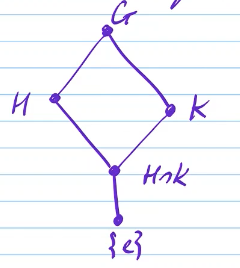
\includegraphics[width=0.3\textwidth]{lattice-ex-1.png}
\end{center}
An ascending edge or sequence of edges implies the lower subgroup is contained in the upper.

\begin{example}[Subgroup Lattice for Triangle Symmetries]
	We have the following lattice
	\begin{center}
		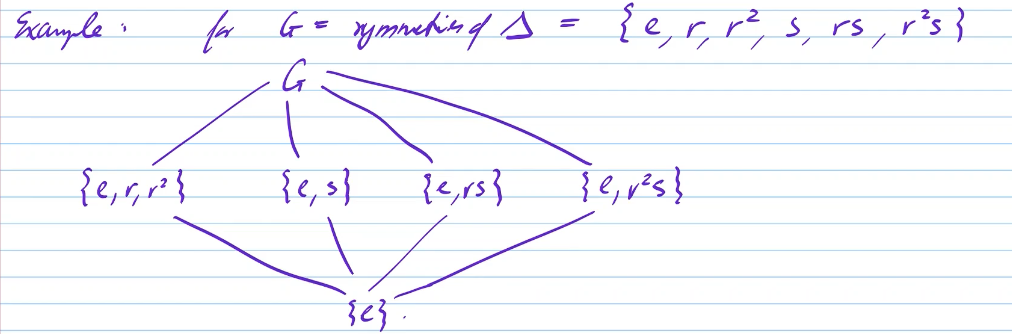
\includegraphics[width=0.8\textwidth]{lattice-ex-2.png}
	\end{center}
\end{example}

\begin{definition}
	Let $X$ be a non-empty subset of a group $G$, then the \vocab{subgroup generated by $X$}, denoted $\langle X \rangle$, is the intersection of all subgroups containing $X$. Equivalently, it is the smallest subgroup of $G$ containing $X$.
\end{definition}



\end{document}
